\subsubsection{Pertinence du découpage}

Je trouve que le découpage choisi par \gil et \damien était une bonne idée. En effet, le projet pourrait s'apparenter à une mission de recherche et développement pour le compte de la \sncf. Ils n'étaient pas certains que leur besoin était réalisable et si la solution utilisée par l'axe sud-est était industrialisable. Ce planning permet de ressentir ces phases de validation du caractère réalisable, puis de création du produit fini.

Le découpage en sous-missions et en lots permet également au client de ne pas trop s'engager dans un projet long terme, et allège aussi la facture -- du moins sur le moment, puisqu'elle sera la même en fin de compte.\\
Cela permet de jouer sur les biais psychologiques du client et paraître moins cher que la concurrence pour obtenir le contrat. \tnp paraît donc proposer des tarifs plus attractifs par rapport aux autres acteurs du marché.

Par ailleurs, ce planning s'inscrit dans les recommandations du 
\gls{agile}\footnote{\glsdesc{agile}.}\cite{noauthor_4_nodate}\cite{noauthor_manifeste_nodate}
, et notamment dans son implémentation par l'ensemble de bonnes pratiques
\gls{scrum}\footnote{\glsdesc{scrum}.}\cite{noauthor_scrum_nodate}.

En effet, le client est impliqué dans la conception du produit tout au long de la mission grâce aux réunions hebdomadaires, et le développement est découpé en courtes périodes que l'on pourrait qualifier de \textit{sprints}.

Cette organisation de travail permet à l'équipe d'avoir des retours réguliers sur le travail produit d'une part, et de récupérer des les informations nécessaires au fil du développement d'autre part. Pour le client, c'est aussi une manière de le rassurer et de voir l'évolution en temps réel pour ne pas perdre patience.

En dernier lieu, le développement agile des projets est à la mode, et infiniment plus confortable pour les clients qui peuvent désormais demander à leurs prestataires d'être plus flexibles que dans une gestion de projet plus traditionnelle.\\
Ce modèle tend à devenir la nouvelle norme, et dans un marché aussi concurrentiel la \df se devait de s'y confirmer.

\subsubsection{Respect du planning}

Le projet a pris du retard dès la conception des \gls{poc}. Aussi bien pour la partie \ds que chez les développeurs.

Le client envoyait régulièrement les données mises à jour des différentes sources \sncf à l'équipe \ds. Leur format avait tendance à varier ou évoluer, par conséquent les \ds devaient retravailler leurs traitements.

De plus, pour chaque source il fallait en comprendre tous les rouages afin de synthétiser l'information au mieux. Cette partie était délicate, puisque trouver l'information n'était pas une tâche aisée.

De notre côté, chez les développeurs, nous avions sous estimé le temps que prendrait la compréhension des données d'une part, mais également celle des règles des anomalies, la bibliothèque des écarts. En effet, cette dernière utilisait des critères non explicites dans l'outil de l'axe sud-est.

Si bien qu'il a fallu à un moment se créer un tableau de synthèse de nos données pour les comparer avec le résultat obtenu sur l'outil du client. Grâce à ce tableau, nous avons pu trouver l'existence de ces critères et corriger notre implémentation de la bibliothèque des écarts.

L'équipe \ds nous a également été d'une aide précieuse, puisqu'ils avaient effectué ce travail de compréhension des données avant nous.

Enfin, comme expliqué précédemment, les mouvements sociaux de décembre 2019, et la crise du \textsc{COVID-19} ont ralenti le déroulement du projet.

\newpage
\subsubsection{Améliorations possibles}

 Bien que cela aille à l'encontre d'une des valeurs du \gls{agile}, je pense qu'une meilleure documentation de l'existant de la part du client nous aurait aidés à avancer plus rapidement. Souvent, lors de la réalisation du projet, nous manquions d'explications plus claires et précises sur le fonctionnement de l'outil de bouclage de production existant.
 
 Certaines données n'étaient pas très explicites, et c'était d'autant plus le cas pour les règles de la bibliothèque des écarts permettant de donner un statut aux trains.
 Si bien que nous avons créé notre propre documentation du projet existant pour centraliser l'état de nos connaissances. Nous notions par exemple le sens des différentes données, et les critères réellement utilisés dans les règles lib-écarts.

\begin{figure}[H]
  \centering
  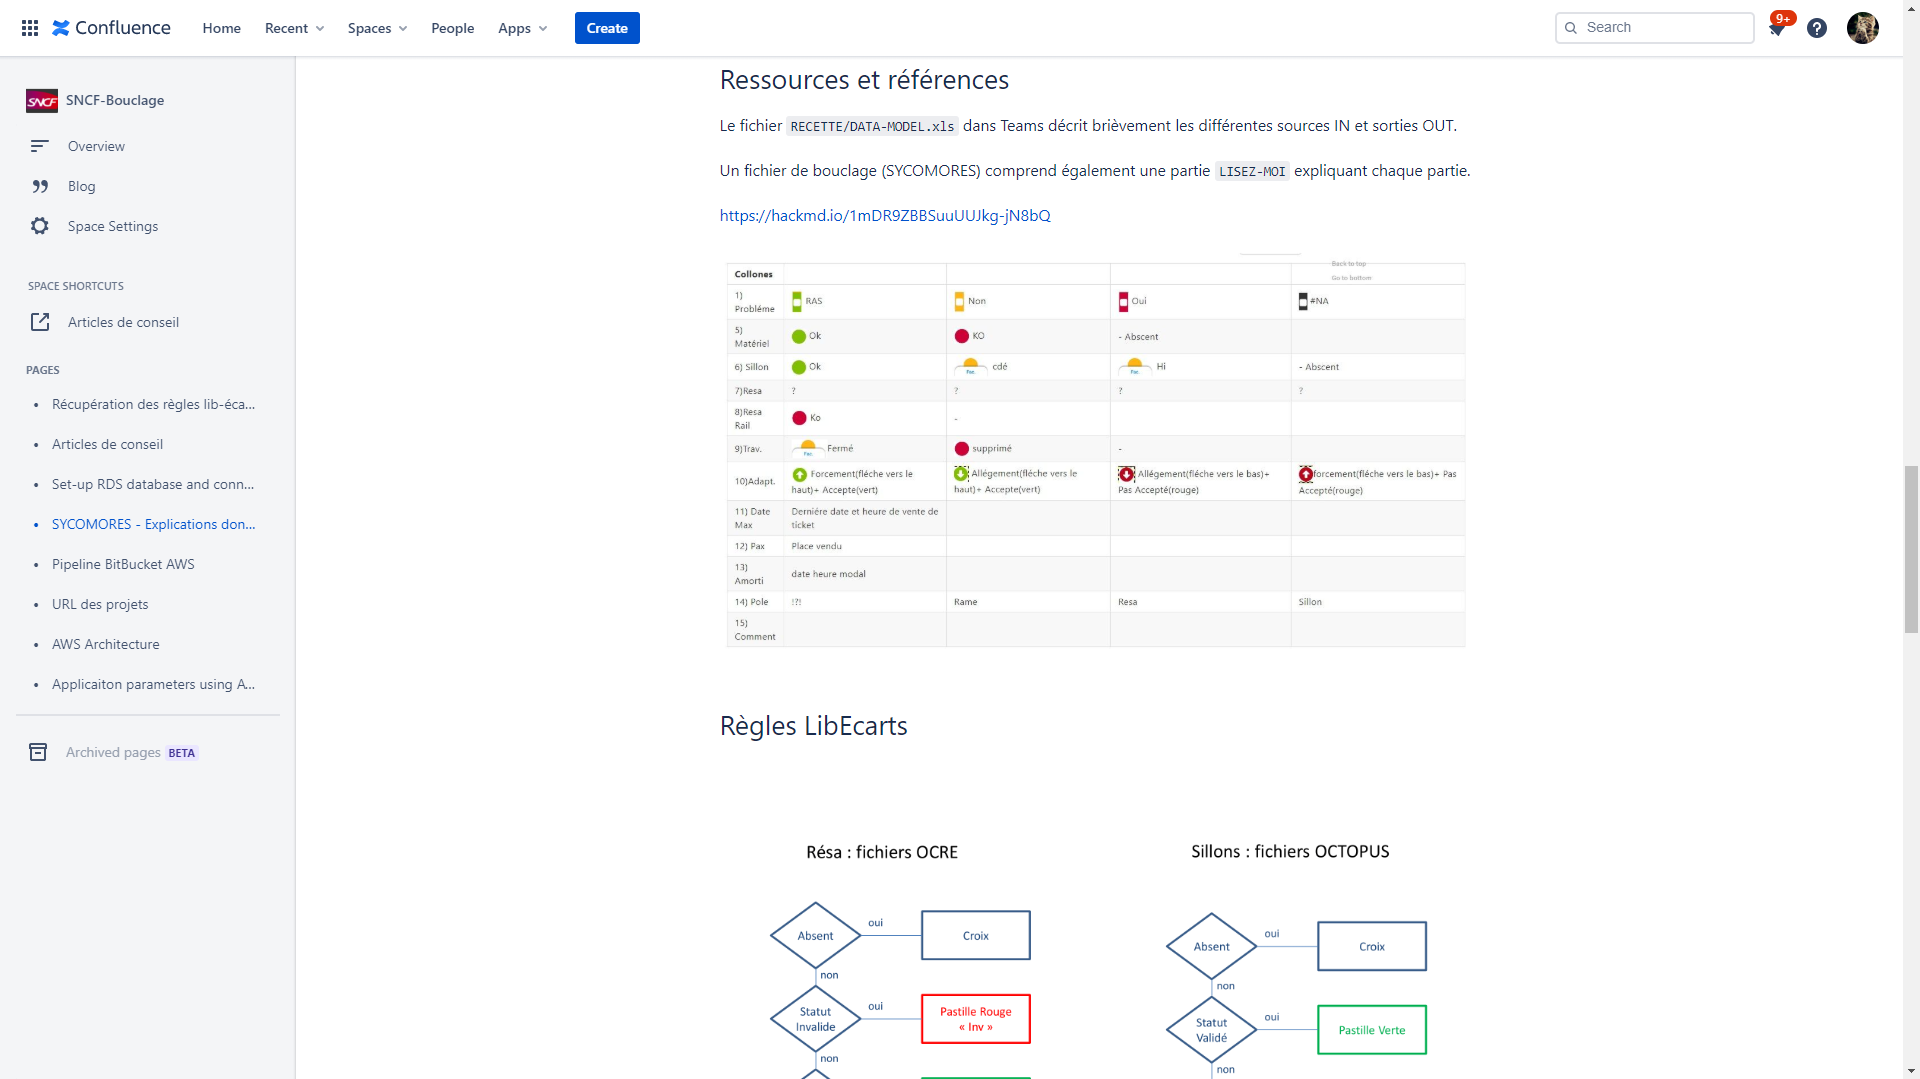
\includegraphics[width=1\linewidth]{img/confluence_sycomores_explications.png}
  \caption{Page Confluence recensant nos connaissances à propos du projet existant de l'axe sud-est}
\end{figure}

Ce travail aurait pu être effectué en amont du projet avec le client ou bien fourni par ce dernier. Le \gls{agile} n'est d'ailleurs pas complètement opposé aux documentations. Il est surtout question de donner aux développeurs des tâches claires et simples et de ne pas s'attarder sur la documentation de ce qu'ils conçoivent, mais plutôt sur les fonctionnalités apportées. Créer ou récupérer une documentation claire en amont n'aurait pas forcément été à l'encontre de cela, même si le planning et le projet sont flexibles.

Ceci dit, ce manque de transparence était possiblement dû à une réticence au changement de la part de la personne en charge de l'outil utilisé chez \sncf. En effet, une seule personne s'occupait de maintenir à jour les macros et les exécuter. Une façon de pallier ce problème aurait été d'intégrer cette personne aux ateliers lors de la première phase du projet, pour la rendre actrice de la mission.

\subsubsection{Le manifeste agile et la méthode \textit{Scrum}}

La méthode \gls{scrum} est adaptée aux projets de développement informatique actuels. Cependant, les principes du \gls{agile} sont, à mon sens, parfois utilisés comme prétexte par les clients pour gagner du pouvoir sur les prestataires. Pour rappel, le \gls{agile} promeut, entre autres, un planning adaptable, un développement de logiciels évolutif, et une grande ouverture au changement.

Cela a bien des vertus lors d'un projet, mais cette flexibilité créer un déséquilibre dans la relation entre le client et le prestataire de services. Sous couvert de la flexibilité que ce dernier se doit d'avoir, le client lance des projets en se disant qu'il pourra les faire évoluer dans tous les cas, et en profite même parfois pour ajouter de lourdes modifications au projet sans revoir le chiffrage initial.

En travaillant dans un cabinet de conseil, c'est le point qui m'inquiète le plus dans la gestion de projet. \damien a toujours su gérer le client pendant le projet, mais c'est une pression qui pèse sur le chef de projet en plus de sa charge de travail habituelle.